\chapter{\label{chap:state-of-the-art}State of the Art}
In this chapter we describe existing algorithms, protocols and applications in computer science, which try to solve, or give an alternative for, the centralized power in Big Tech, and more specifically in digital audio streaming. We inspect full solutions in the form of distributed applications, and techniques which solve subproblems, such as decentralized file sharing protocols.

For an application to evolve without a company or a responsible group of people, decisions need to be made on protocol or feature additions and changes. We inspect the state-of-the-art technologies and organizational theories which enable autonomous communities to solve these problems by organizing themselves.

\section{Decentralized Autonomous Organizations}
As an alternative organizational framework for distributing money and music, we examine a recent concept and technology: Decentralized Autonomous Organizations (DAO).
A DAO is ``an entity that lives on the internet and exists autonomously, but also heavily relies on hiring individuals to perform certain tasks that the automaton itself cannot do''~\citep{buterin2014dao}. It is not owned by a single person or legal entity. It should also not require a specifically specified party to operate. For example, it should not depend on a single server or database, but rather have flexibility in adopting resources. As such we say it lives \textit{autonomously}. \cite{buterin2014dao} also notes that a DAO should have \textit{internal capital}: `some kind of internal property that is valuable in some way, and it has the ability to use that property as a mechanism for rewarding certain activities'. A DAO is non-profit by nature, as there is no legal owner of the system. Examples of DAOs deployed in the real world are Bitcoin and Ethereum.

Important groundwork around the theory and implementation of a DAO has been done by \cite{jentzsch2016decentralized}. He notes that corporations originally work through people only, and this has two flaws: ``People do not always follow the rules, and they do not always agree what the rules require''. His paper illustrates a method that allows creating and maintaining organizations in which ``(1) participants maintain direct real-time control of contributed funds and (2) governance rules are formalized, automated and enforced using software''.

\section{AI DAO}
Central to this thesis is the real-world experimentation of an intelligent decentralized system: a system that is on the boundary of DAO and AI technologies (see \ref{fig:dao-quadrants}). This means humans are still involved with performing some tasks and governing, but an intelligent agent can perform other decision making tasks. This may be the holy grail in automation. In our context, we envision human tasks to be: creating music and giving feedback on music (through e.g. donations). 'Robot tasks' could be: processing an automatic subscription payment system, in which all user money is divided fairly over the artists every month.

Much is still unknown in this research area. This thesis aims to create more knowledge on a 'AI DAO' by attempting to build a proof-of-concept of such intelligent system.

\begin{figure}
    \centering
    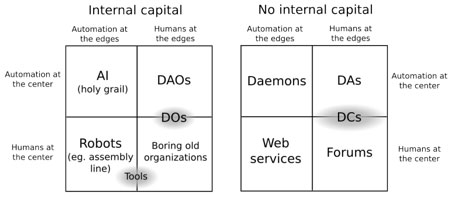
\includegraphics[width=0.7\textwidth]{introduction/dao-quadrants.jpg}
    \caption{Decentralized Autonomous Organization, in comparison to other organizational structures. In a DAO, activity is performed by humans at the edges, automation at the center. It is an interplay in which robots and humans perform tasks. Source: \cite{buterin2014dao}}
    \label{fig:dao-quadrants}
\end{figure}

\section{Decentralized music distribution technologies}
Multiple decentralized audio distribution and streaming applications exist. Examples are Audius~\citep{audius2018}, Musicoin~\footnote{\url{http://musicoin.org/}} and Opus Audio~\citep{jia2016opus}.

\subsection{Audius}
Audius~\citep{audius2018} presents a decentralized protocol for audio content, which aims to improve payouts to artists and its transparency. It contains a token economy with a transparent payout system for the artists, and a user-operated, distributed network for metadata and content. In addition, it has a governance system like a DAO, in which users can decide on changes to the protocol by democratic voting. Its protocol is established around the ideology of disintermediation: ``Intermediaries  should  be  removed  when  possible; when necessary, they should be algorithmic, transparent, and verifiably accurate''~\citep{audius2018}. It uses IPFS~\citep{benet2014ipfs} for storage of audio content, meaning it relies on voluntarily-hosted high-performant servers.

\subsection{Opus Audio}
Opus Audio~\citep{jia2016opus} is a decentralized music-sharing platform and proposes a solution for music ownership registration on a blockchain structure. It has a running distributed audio file sharing system using the Inter-Planetary FileSystem designed by \cite{benet2014ipfs} (see \ref{sec:decentralized-content-delivery}). It contains a decentralized and fully automated system for purchasing access to music, which works as follows. Opus stores encrypted audio files on a swarm of connected nodes. The decryption keys and files hashes are stored in a smart contract (see \ref{sec:smart-contracts}). Using cryptocurrency, users spend their funds on these smart contracts, to unlock access to audio files.

\subsection{Musicoin}
Musicoin is a blockchain platform without intermediaries that focuses on income for independent artists. It uses smart contracts and cryptocurrency to show transparency in payments (see \ref{sec:smart-contracts}). This payment structure ensures that each contributor in the network is rewarded, and that artists receive a stable income based on the Universal Basic Income ideology. Not all of their architecture is decentralized; they use centralized registration system for artists and listeners. They pay artists using their \$MUSIC currency, of which the value may be highly unstable.

\subsection{Comparison}
None of the state-of-the-art decentralized audio streaming technologies show a running, fully decentralized infrastructure with stable income for artists. All of these systems have in common that they save metadata and identifiers of audio files on a blockchain, and save the audio files in an off-chain database using IPFS~\citep{benet2014ipfs}. This makes these solutions reliant on people voluntarily running IPFS content nodes (servers hosting the audio files). In a fully decentralized network, every participant should have the same role, meaning that every node both uploads and downloads content, and it should not be reliant on external servers. Most decentralized systems use their homebrew cryptocurrency to pay artists, instead of a well-established currency or stablecoin. 

\section{Transparent, automated royalty distribution}
\label{sec:smart-contracts}
The payment to royalties to artists can be described in a transparent and immutable record on a blockchain. In addition, smart contracts can be used to automate payments~\citep{buterin2014next}. Smart contracts are self-executing (no ambiguity) and self-verifying (guaranteeing its statements). In the music industry context, a smart contract can be used for transparent, immutable and automatic payment distribution of royalties. This technique was shown in practice in 2017, when Imogen Heap released the song `Tiny Human'~\citep{heap2017blockchain}. Its distribution of payments to the makers and recorders was written in a smart contract, in the form of a record on the Ethereum blockchain. When a user downloads the corresponding track and makes the payment using cryptocurrency, the forwarding details of the payment are located within the blockchain, and executed as declared on the smart contract.

\section{Decentralized application frameworks}
\label{sec:sote-trustchain}
The TrustChain superapp~\citep{mattskala2020} is a framework for implementing mobile Android decentralized applications. It allows for storing append-only immutable data on TrustChain~\citep{otte2017trustchain} and spreading this data in a phone-to-phone serverless network. It follows the concept of super apps~\citep{kpmg2019superapps}, meaning that it contains many mini-apps which use the same networking interface. The Superapp is an Android app as seen in fig. \ref{fig:trustchain-superapp}. Its mini-apps implement decentralized democratic voting and has bitcoin payment integration, among other features.

\begin{figure}
    \minipage{0.3\textwidth}
        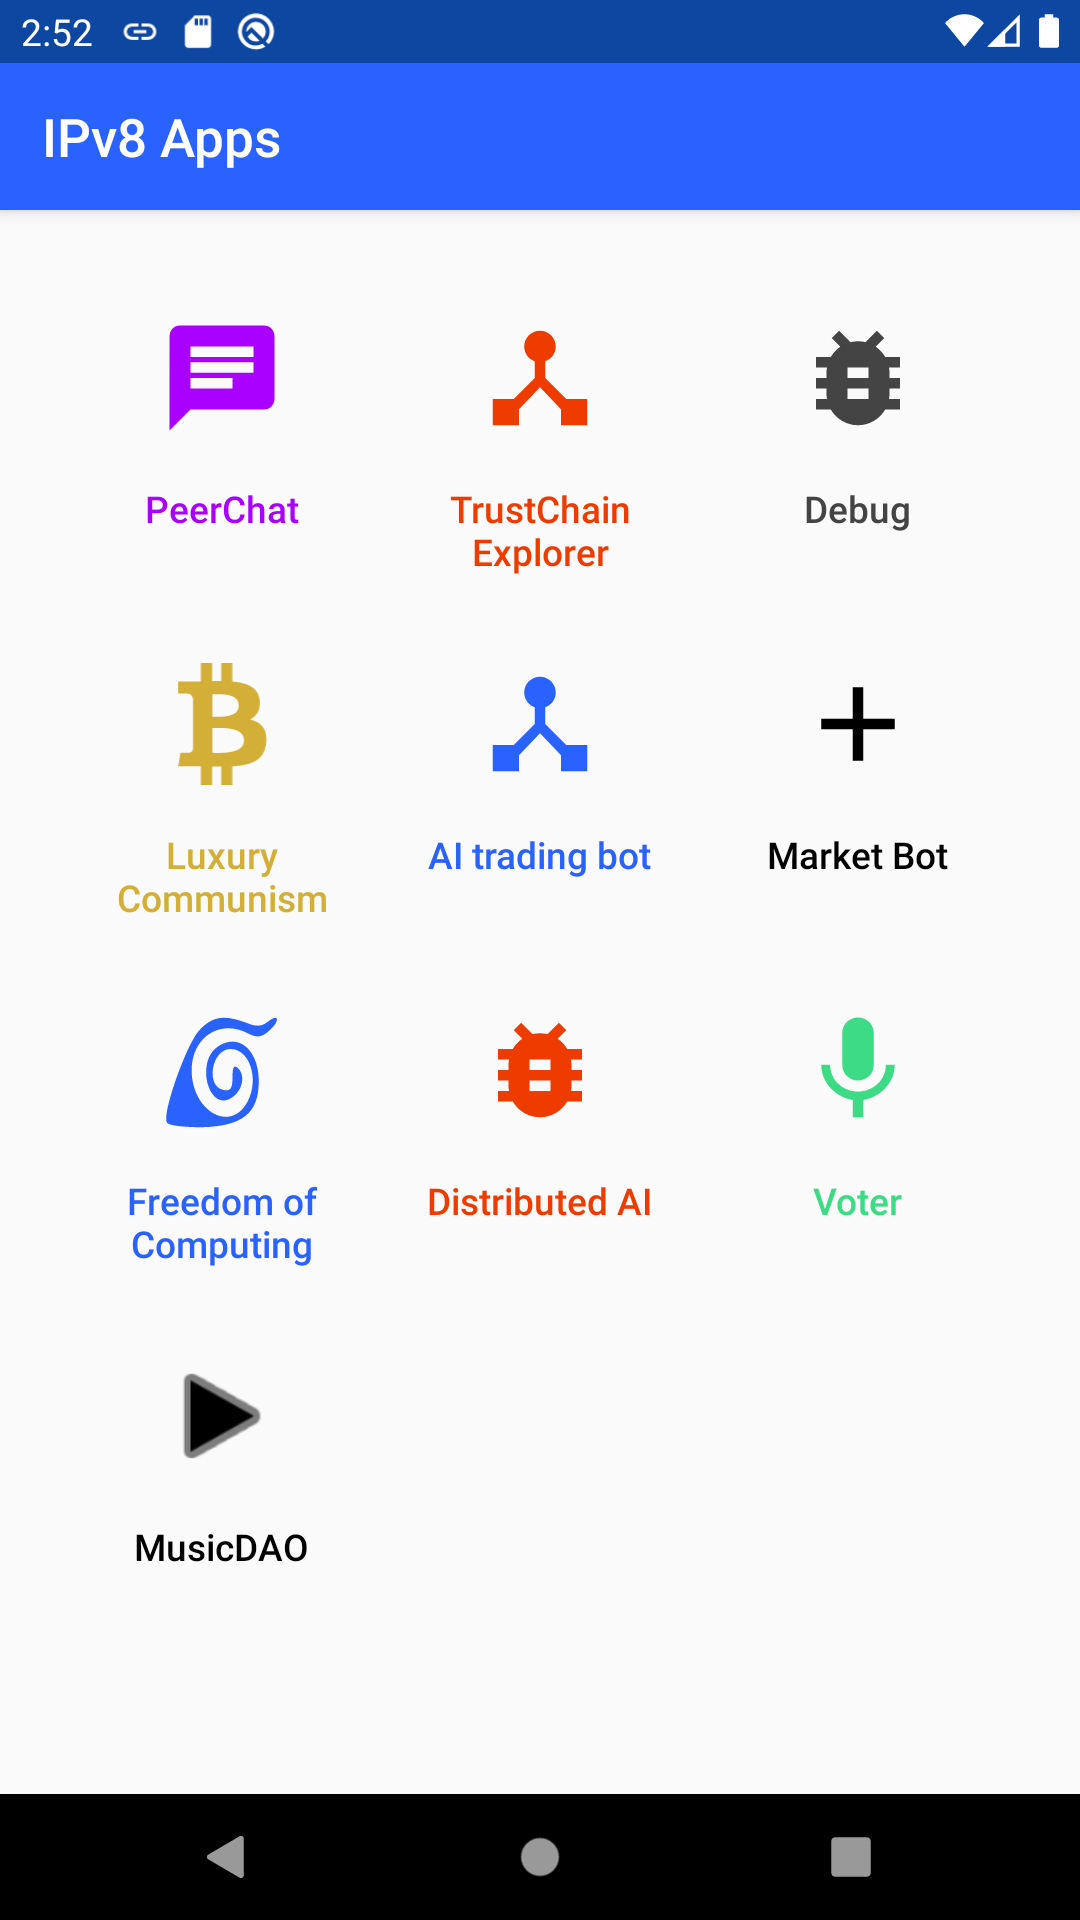
\includegraphics[width=1\linewidth]{related-work/screenshot-superapp.png}
        \caption{Trustchain-Superapp overview}
        \label{fig:trustchain-superapp}
    \endminipage\hfill
    \minipage{0.65\textwidth}
        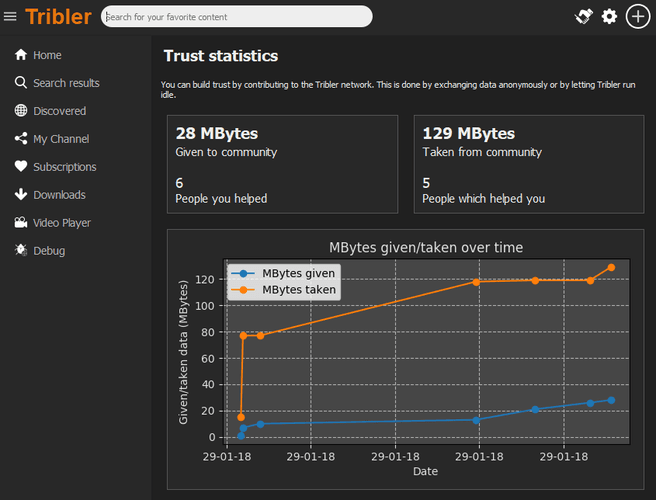
\includegraphics[width=1\linewidth]{related-work/tribler7.3.0.png}
        \caption{Tribler desktop interface, showing the bandwidth incentive system overview}
        \label{fig:tribler}
    \endminipage
\end{figure}

In the context of DAO, the TrustChain-Superapp contains a mini-app for decentralized governance using voting (see fig. \ref{fig:trustchain-superapp-voter}). In this voting app, any participant of the organization can create a proposal for the community to vote on. Once a preset voting threshold is reached, the proposal is automatically accepted or denied. Bookkeeping of these proposals is done using the TrustChain distributed ledger technology~\citep{otte2017trustchain}. This voting app is an important basis for democratic decision making, but does not include code changes directly after proposals are accepted, so lacks app evolution. This protocol is based on proof-of-identity instead of proof-of-stake, as no tokens are involved.

\begin{figure}
    \centering
    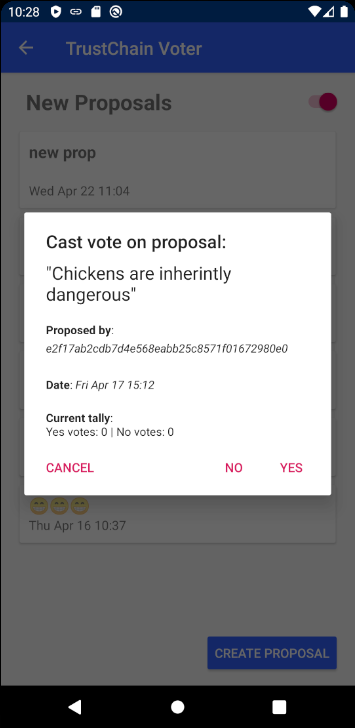
\includegraphics[width=0.3\linewidth]{related-work/trustchain-superapp-voter.png}
    \caption{Distributed democratic voting mini-app, showing proposals}
    \label{fig:trustchain-superapp-voter}
\end{figure}

\section{Decentralized content delivery networks}
\label{sec:decentralized-content-delivery}
A fully decentralized audio streaming service requires sharing and streaming audio files over a network of nodes in which any participant can start and run a node. Well-established examples of such technologies are BitTorrent and IPFS.

\subsection{BitTorrent}
BitTorrent~\citep{cohen2002bittorrent} is an open peer-to-peer file sharing protocol. It invented by Bram Cohen, and has generated a massive influence on network traffic on the Internet since its release. Today, it is still the most popular peer-to-peer protocol for sharing data. In 2019, BitTorrent was measured to generate 2.5\% of all download and 24.6\% of all upload bandwidth~\citep{marozzo2020}. It went through many iterations and improvements. It has a large community, with over 3K repositories on GitHub related to the technology. Furthermore there are a few companies maintaining clients (such as \url{https://bittorrent.com} and \url{https://www.utorrent.com}).

In essence, BitTorrent makes use of seeding while downloading: this means that when multiple clients download a file, they simultaneously share pieces of this file with the other downloaders. This results, with well connected and performing peers, in fast downloads. 
% A key challenge is finding and connecting to healthy \textit{swarms}: groups of uploaders and downloaders that are interested in some piece of content.

% he BitTorrent file distribution system uses tit-for-tat as a method of seeking pareto efficiency

% Any person can join the network and start sharing files, by making a torrent which contains the metadata of the files. Content is specified using SHA1 hashes of the files. Checksums are used to make sure no changes to the original torrent have been made upon receiving files. This way all files are immutably shared. BitTorrent has implementations for various systems, including Android. This means mobile devices can participate in uploading and downloading content, and can even build an autonomous phone-only file sharing system.

% Torrent files contain a list of chunks (torrent pieces), which represent the different parts of the related file. Flawless streaming of media files over BitTorrent requires a smart algorithm to predict what file is requested next, and what torrent pieces should be loaded. 

% BitTorrent originally relied on trackers to perform peer discovery, and trackers can become a central point of failure. However, since the introduction of the DHT protocol~\citep{bittorrentbep5dht}, finding peers in the network can be done by querying any known peer, which makes the network more decentralized. 

There are no differences between hosters and downloaders. All participants have the same capabilities, so every user of the network can both download and upload content. A challenge of the BitTorrent protocol without extensions is incentivizing participants to host files. There are multiple proposed solutions for this, discussed in \ref{sec:file-spreading-incentives}.

\subsection{IPFS}
The Inter-Planetary FileSystem, introduced by \cite{benet2014ipfs}, is a distributed peer-to-peer file sharing system in which any person can start a node and start uploading and downloading files. Protocol Labs\footnote{\url{https://protocol.ai/}}, the team behind this technology, was founded in 2014 by Juan Benet. As of 2020, the team has grown globally to members from 19 countries, with substantial investments. However, there has not been large-scale adoption of this technology yet.

% It uses a Distributed Hash Table to address content using a combination of SHA-256 hashes and hyperlinks. 

At its core, IPFS maintains a global key-value store for all files (and file parts). This is in contrast to BitTorrent, which works with torrent swarms and trackers. IPFS uses an efficient content addressing mechanism. Another feature is built-in file de-duplication. Additionally it supports public file history bookkeeping.

End-users of content stored on IPFS can access content without supporting the network, so there is the possibility of free-riding. In addition, there are no direct (financial) incentives to run an IPFS node, other than to help the network and to host content. 
% For example, users of the aforementioned Audius music streaming system are not required to run an IPFS node to improve the health of the network. 
\subsection{Comparison: IPFS and BitTorrent}
A notable difference between IPFS and BitTorrent is that IPFS makes a difference in file-hosting nodes and end-users (which only download files). BitTorrent does not make a distinction between these actors. In BitTorrent, every participant of the network has the capabilities to both upload and download content. Therefore a BitTorrent network using DHT is typically more decentralized than IPFS. 

IPFS uses a global file index using a hash tree, which means that every two file that produce the same hash are stored on the same index. This leads to de-duplication, which may result in better use of disk space, in comparison to BitTorrent.

% \begin{figure}
%     \minipage{0.45\textwidth}
%         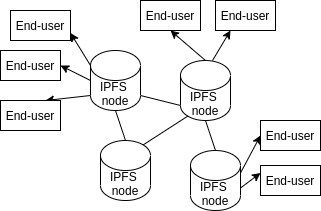
\includegraphics[width=1\linewidth]{related-work/decentralized-ipfs.png}
%         \caption{Decentralized file sharing structure: each node hosts nodes for some end-users}
%         \label{fig:decentralized}
%     \endminipage\hfill
%     \minipage{0.45\textwidth}
%         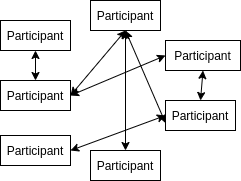
\includegraphics[width=1\linewidth]{related-work/distributed-bittorrent.png}
%         \caption{Distributed file sharing structure: each participant can exchange with each other participant}
%         \label{fig:distributed}
%     \endminipage
% \end{figure}

\section{Incentives for file hosting}
\label{sec:file-spreading-incentives}
In a DAO, the party responsible for hosting and spreading of files is not well-defined. To tackle the tragedy of the commons, entities should be incentivised just enough for the system to be sustainable and usable, but no more. An example incentive system is bandwidth tokens~\citep{de2018blockchain} as part of the Tribler system.

Tribler~\citep{pouwelse2008tribler} is a peer-to-peer system to share, download and stream multimedia. It has implementations for desktop environments and an Android prototype. It makes use of BitTorrent for file transfer and adds anonymization techniques on top of it. In addition, it makes use of its bandwidth tokens: an incentive system to increase cooperation between users, in order to achieve high availability of downloads. In essence, it subtracts tokens for downloading content from peers and rewards tokens for helping peers. An overview of the Tribler desktop interface can be seen in fig. \ref{fig:tribler}.

% FileCoin

% TODO READ/DISCUSS FOLLOWING RELATED WORK:
% https://github.com/javto/Tribler-streaming
% Decentralized Media Streaming on Android using Tribler

% STEEM
% PeerTube